%%%%%%%%%%%%%%%%%%%%%%%%%%%%%%%%%%%%%%%%%
% Beamer Presentation
% LaTeX Template
% Version 1.0 (10/11/12)
%
% This template has been downloaded from:
% http://www.LaTeXTemplates.com
%
% License:
% CC BY-NC-SA 3.0 (http://creativecommons.org/licenses/by-nc-sa/3.0/)
%
%%%%%%%%%%%%%%%%%%%%%%%%%%%%%%%%%%%%%%%%%

%----------------------------------------------------------------------------------------
%	PACKAGES AND THEMES
%----------------------------------------------------------------------------------------

\documentclass[10pt]{beamer}

\mode<presentation> {

% The Beamer class comes with a number of default slide themes
% which change the colors and layouts of slides. Below this is a list
% of all the themes, uncomment each in turn to see what they look like.

%\usetheme{default}
%\usetheme{AnnArbor}
%\usetheme{Antibes}
%\usetheme{Bergen}
%\usetheme{Berkeley}
%\usetheme{Berlin}
%\usetheme{Boadilla}
%\usetheme{CambridgeUS}
%\usetheme{Copenhagen}
%\usetheme{Darmstadt}
%\usetheme{Dresden}
%\usetheme{Frankfurt}
%\usetheme{Goettingen}
%\usetheme{Hannover}
%\usetheme{Ilmenau}
%\usetheme{JuanLesPins}
%\usetheme{Luebeck}
%\usetheme{Madrid}
%\usetheme{Malmoe}
%\usetheme{Marburg}
%\usetheme{Montpellier}
%\usetheme{PaloAlto}
%\usetheme{Pittsburgh}
\usetheme{Rochester}
%\usetheme{Singapore}
%\usetheme{Szeged}
%\usetheme{Warsaw}

% As well as themes, the Beamer class has a number of color themes
% for any slide theme. Uncomment each of these in turn to see how it
% changes the colors of your current slide theme.

%\usecolortheme{albatross}
%\usecolortheme{beaver}
%\usecolortheme{beetle}
%\usecolortheme{crane}
\usecolortheme{dolphin}
%\usecolortheme{dove}
%\usecolortheme{fly}
%\usecolortheme{lily}
%\usecolortheme{orchid}
%\usecolortheme{rose}
%\usecolortheme{seagull}
%\usecolortheme{seahorse}
%\usecolortheme{whale}
%\usecolortheme{wolverine}

%\setbeamertemplate{footline} % To remove the footer line in all slides uncomment this line
\setbeamertemplate{footline}[page number] % To replace the footer line in all slides with a simple slide count uncomment this line

\setbeamertemplate{navigation symbols}{} % To remove the navigation symbols from the bottom of all slides uncomment this line
}

\usepackage{graphicx} % Allows including images
\usepackage{booktabs} % Allows the use of \toprule, \midrule and \bottomrule in tables
\usepackage{listings}

%----------------------------------------------------------------------------------------
%	TITLE PAGE
%----------------------------------------------------------------------------------------

\title[DDP]{Attack on ROB and Prefetcher} % The short title appears at the bottom of every slide, the full title is only on the title page

\author{Meet Udeshi, Nirmal Boran\\
Prof. Virendra Singh} % Your name
\institute[CADSL] % Your institution as it will appear on the bottom of every slide, may be shorthand to save space
{
CADSL - IIT Bombay\\ % Your institution for the title page
}
\date{\today} % Date, can be changed to a custom date

\begin{document}

\begin{frame}
\titlepage % Print the title page as the first slide
\end{frame}


\section{ROB based Side Channel}
\begin{frame}
\frametitle{Hypothetical ROB based Side Channel}
\begin{itemize}
    \item Reorder buffer is used by Out-of-Order cores for in-order retirement.
    \item In SMT cores, fairness policy ensures that roughly equal instructions are retired for all threads to maintain equal IPC.
    \item Simple implementation is to share retire pipeline width equally among threads.
    \item But when one thread is stalled, other thread will use full pipeline width to retire.
    \item IPC of other threads will see a slight increase.
    \item Data-dependent branch misses and cache misses can be infered from IPC information.
\end{itemize}
\end{frame}

\begin{frame}
\frametitle{Hypothetical ROB based Side Channel}
\begin{figure}
\centering
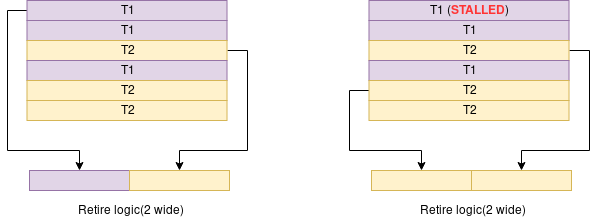
\includegraphics[width=0.8\textwidth]{rob_side_channel}
\caption{Reorder buffer for SMT. When T1 is stalled T2 retires twice as many instructions.}
\end{figure}
\end{frame}

\begin{frame}
\frametitle{Disabling Prefetcher to avoid Cache Pollution}
\begin{itemize}
\item Cache side-channels work by extracting information about cache accesses of victim process
\item Any other process or hardware block which accesses the cache will increase noise in the side-channel
\item Fuchs et al. \footnote{Disruptive prefetching: impact on side-channel attacks and cache designs - SYSTOR'15} have proposed a method to make prefetcher increase noise in cache and disrupt cache side-channel attacks
\item We propose to disable the prefetcher by not allowing it to learn the stride patterns
\item This can be done by running a third process in parallel which makes random loads
at PC which alias with victim process' load PCs
\end{itemize}
\end{frame}


\begin{frame}
\Huge{\centerline{The End}}
\end{frame}


%----------------------------------------------------------------------------------------

\end{document}
